\begin{itemize}
    \item Fourier Transform (theoretisches tool, weil digital nicht umsetzbar): kernel, eigenschaften (linear, shift, skalierung), beispiele uebung 
    \item Discrete Time Fourier Transform (theoretisches tool, weil digital nicht umsetzbar)
    \item Discrete Fourier Transform
    \begin{itemize}
        \item eigenschaften der kernel-funktion: perioden, wann reel, ..., was passiert bei abtastung?
        \item implizite periodifizierung des signals?
        \item zusammenhang zur physik
        \item dc, nyquist-frequenzen, wann vorhanden?
        \item reelles signal: dc und nyquist reell
    \end{itemize}
    \item zusammenhang zwischen ft, dtft und dft (intuition mit periodifizierung vs. abtastung; non-intuition durch kernel angucken)
    \item dft als approximation der ft
    \begin{itemize}
        \item $s(t) = \exp(-t/\tau) \cdot \sin(\omega_0 \cdot t)$, 
        \item $s(t) = \exp(-(t - \mu)^2/\sigma^2)$ (Uebung)
    \end{itemize}
    \item spectral leakage;
\end{itemize}
\subsection{Anwendung der Transformationen}
\begin{itemize}
    \item fft (Uebung 1 jup, uebung 2 8.3.2)
    \item bild-kompression (DCT, JPEG)
    \item fensterung \footnote{\url{https://docs.scipy.org/doc/scipy/reference/signal.windows.html}}
    \item schnelle faltung (cyclic/non-cyclic)
    \item beliebig lange signale overlap add, overlap save (\"Ubung: irgendwas mit audio prosessing)
    \item Unschaerfe Relation (Fensterbreite vs. Frequenzaufloesung)\cite[chpt. 4.2]{mallat2008wavelets}
\end{itemize}
%
%
\subsection{DFT-Interpolation}\label{dftintp}
%
% !TEX root = ../dsv_script.tex
%
%
\subsubsection{Theoretische Grundlagen}\label{sec:dftintp:theory}
%
Gegeben sei ein periodisches, analoges Signal $x: \R \rightarrow \C$, mit Periode $T_p = 1/F_0$. 
Wir beobachten dieses Signal auf einem uniformen Raster von Punkten, via $x[n] = x(n T)$ und wollen eine Funktion $y(t)$ herleiten, f\"ur welche die Interpolationsbedingung
\begin{equation}\label{eq:dftintp:interpol_cond}
    y(nT) = x[n] = x(nT)
\end{equation}
erf\"ullt ist. 
Hierzu entwickeln wir das Signal $x$ in seine Fourier-Reihe via
\begin{equation}\label{eq:dftintp:fourier_series}
    x(t) = \Sum{k=-\infty}{+\infty}{
        c[k] \exp(\jmath 2 \pi k t F_0) 
    }.
\end{equation}
Nun tasten wir dieses Signal uniform mit Samplerate $F_s = N/T_p = 1/T$ (also passend zur Periodendauer) ab und erhalten die Folge 
\begin{equation}
    x[n] = x(n T) = \Sum{k=-\infty}{+\infty}{
        c[k] \exp(\jmath 2 \pi k n T F_0) 
    } = \Sum{k=-\infty}{+\infty}{
        c[k] \exp\left(\jmath 2 \pi k \frac nN\right) 
    }
    \Text{f\"ur}
    n \in \N
\end{equation}
bestehend aus den Samples von $x$. 
Mit der Periodizit\"at von $\exp(\jmath 2 \pi t)$, siehe \Cref{sec:fourier:disc_period} und \Cref{sec:sampling:disc_sin}, und der Abtastung erhalten wir au{\ss}erdem noch
\begin{equation}
    x[n] = \Sum{k=0}{N-1}{
        \left[\Sum{\ell=-\infty}{+\infty}{
            c[k - \ell N]
        }\right] \exp\left(\jmath 2 \pi k \frac nN\right) 
    } = \Sum{k=0}{N-1}{
        \tilde{c}[k] \exp\left(\jmath 2 \pi k \frac nN\right) 
    },
\end{equation}
wobei wir 
\begin{equation}\label{eq:dftintp:aliased_ck}
    \tilde{c}[k] = \Sum{\ell=-\infty}{+\infty}{
        c[k - \ell N]
    }
\end{equation}
als Abk\"urzung benutzt haben. 
Wir nehmen nun aus guten Grund noch an, dass die Funktion $x$ auch bandbegrenzt ist.
Das hei\"st, ihre Fourier-Transformierte $X : \R \rightarrow \C$ verschwindet au{\ss}erhalb eines gewissen Bandes, also
\begin{equation}
    X(F) = \Int{-\infty}{+\infty}{x(t) \exp(-\jmath 2 \pi F t )}{t} = 0 \Text{f\"ur} \Abs{F} > B.
\end{equation}
Au{\ss}erdem wissen wir, dass die Fourier-Transformation $X$ und die Folge $c[k]$ verkn\"upft sind via 
\begin{equation}
    c[k] = \frac{1}{T_p} X(k F_0),
\end{equation}
was impliziert, dass die Folge $c[k]$ ab einem gewissen $k > K_0$ verschwindet.
Es gilt also
\begin{equation}
    c[k] = 0 \Text{f\"ur} \Abs{k} > \left\lceil \frac{B}{F_0} \right\rceil.
\end{equation}
Das hei{\ss}t, dass wir nun $F_s = N/T_p$ so gro{\ss} w\"ahlen m\"ussen, dass sich in \eqref{eq:dftintp:aliased_ck} kein Aliasing f\"ur $\tilde{c}[k]$ ergeben kann.
Es muss also gelten
\begin{equation}
    N > \lceil B/F_0 \rceil \Text{bzw.} F_s > \lceil B/(F_0 T_p) \rceil.
\end{equation}
Es folgt dann, dass $c[k] = X[k]$, wobei $X[k]$ die \gls{dft} der Folge $x[n]$ darstellt. 
Das hei\"st, dass wir die Fourier-Koeffizienten der kontinuierlichen Funktion $x$ durch die \gls{dft} der Abtastwerte $x[n]$ bestimmen k\"onnen. 
Mit \eqref{eq:dftintp:fourier_series} k\"onnen wir also die Folge $x[n]$ interpolieren, indem wir
\begin{equation}\label{eq:dftintp:dft_interpolation}
    y(t) = \frac{1}{T_p}\Sum{k=-\frac{B}{F_0}}{+\frac{B}{F_0}}{
        X[k] \exp(\jmath 2 \pi k t F_0) 
    }
\end{equation}
schreiben. 
Dieses $y$ erf\"ullt die Interpolationsbedingung \eqref{eq:dftintp:interpol_cond}, weil wegen der Bandbegrenzung von $x$ und der Periodizit\"at sogar $y(t) = x(t)$ f\"ur alle $t$ gilt.

Man beachte hier, dass nun aus der Folge von diskreten Werten $x[n]$ eine analytische Formel in Form einer \emph{endlichen} Summation entstanden ist. 
Unter der Annahme der Bandlimitierung von $x$ ist diese Interpolation \emph{exakt} und kann effizient implementiert werden, durch die Vorberechnung der Folge $X[k]$ durch die \gls{fft}~\cite{FFTW05} der Folge $x[n]$. 
Eine Anwendung der hier vorgestellten Methode zur Interpolation wird in \cref{sec:eadf} aufgezeigt.
%
%
\subsection{DFT-Interpolation von Antennenantworten}\label{eadf}
%
% !TEX root = ../dsv_script.tex
%
\subsubsection{Motivation}
%
%
Mit jeder Erschlie{\ss}ung von neuen Frequenzbereichen f\"ur die Kommunikation ist es von Interesse das Ausbreitungsverhalten der Elektro-Magnetischen Wellen f\"ur verschiedene Umgebungen zu charakterisieren, beispielsweise innerst\"adtisch, auf der Autobahn, etc. Zwar k\"onnen solche Umgebungen auch computerbasiert simuliert werden, doch f\"ur eine empirisch abgeleitete Statistik solcher sogenannter Kanalmodelle~\cite{delgaldo2007phd} sind repr\"asentative Messungen unerl\"asslich. Diese Charakteristiken werden genutzt, um in realistischen Szenarien Kanalkapazit\"aten, Datenraten und dergleichen zu bestimmen. Schlussendlich flie{\ss}en solche Statistiken dann in neue Mobilfunkstandards ein.

\begin{figure}
    \centering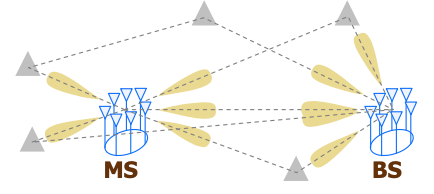
\includegraphics[width=0.6\textwidth]{img/eadf/sounding.png}
    \caption{Schematische Darstellung einer \acrshort{mimo} Kanalmessung. Grafik aus~\cite{richter_estimation_2005}.}\label{eadf_sounding}
\end{figure}

Das FG EMS hat sich deshalb unter anderem auf solche Messungen und deren Auswertung, das sog. Channel Sounding~\cite{thomae2005multidim_hrpe}, spezialisiert. Hierbei kommen meist breitbandige \gls{mimo} Messsysteme zum Einsatz, die den Funkkanal in Frequenz, Raum und Zeit koh\"arent vermessen k\"onnen, wie in \Cref{eadf_sounding} dargestellt. Anschlie{\ss}end nutzt man spezielle Signalverarbeitungstechniken~\cite{semper2023wideband_channel_sounding}, die einerseits unter gewissen physikalischen Annahmen das Ausbreitungsverhalten aus den gemessenen Daten ableiten k\"onnen, und andererseits gleichzeitig den Einfluss des Messsystems so weit wie m\"oglich aus den gesch\"atzten Kanalstatistiken entfernen. Schlie{\ss}lich ist man an der Realit\"at au{\ss}erhalb des Messaufbaus interessiert. 

Nat\"urlich sind hierzu vor der Messung pr\"azise Kalibriermessungen des Systems notwendig. Wir wollen uns im folgenden auf die Wirkung der benutzten Antennenarrays konzentrieren, da diese -- wie wir sehen werden -- eine gewisse Sonderbehandlung ben\"otigen. Zun\"achst stellt man bei der Konzipierung und Benutzung des Messsystems sicher, dass es sich um ein \gls{lti} System handelt. Betrachtet man nun das Verhalten des Systems im Frequenzbereich f\"ur ein einzelnes Paar von Sende- und Empfangsantenne, dann gilt demnach zun\"achst
\begin{equation}
    Y(f) = G_{\rx}(f) \cdot H(f) \cdot G_{\tx}(f) \cdot X(f).
\end{equation}
Hierbei steht $X$ f\"ur die Anregung des Systems durch ein eingegebenes Signal, $G_{\tx/\rx}$ f\"ur die Transferfunktion der Sender- bzw. Empf\"angerhardware, und $H$ f\"ur die Transferfunktion des Funkkanals, der demnach auch als ein \gls{lti} system modelliert wird. Es stellt sich aber heraus, dass jede Antenne eine \emph{winkelabh\"angige} Richtcharakteristik besitzt. Das hei{\ss}t, dass die Systemantworten $G_{\tx/\rx}$ davon abh\"angig sind, in welche Richtungen sich die Wellen vom Sender $\tx$ ausbreiten und aus welchen Richtungen, sie am Empf\"anger $\rx$ eintreffen. 

Um dies korrekt zu modellieren, muss man sich also zun\"achst auf einzelne sog. \emph{Ausbreitungspfade} konzentrieren. Das hei{\ss}t wir nehmen an, dass eine ebene Welle sich in die normierte Richtung $\Omega_{\tx}$ ausbreitet und nach ihrem Weg durch den Funkkanal am Empf\"anger aus normierter Richtung $\Omega_{\rx}$ eintrifft. Folglich ergibt sich f\"ur dieses Verhalten
\begin{equation}\label{eadf_single_path}
    Y(f, \Omega_{\tx}, \Omega_{\rx}) = 
        G_{\rx}(f) \cdot a_{\rx}(f, \Omega_{\rx})
        \cdot H(f, \Omega_{\tx}, \Omega_{\rx}) 
        \cdot a_{\tx}(f, \Omega_{\tx}) \cdot G_{\tx}(f)
        \cdot X(f),
\end{equation}
%
wobei $a_{\tx/\rx}$ f\"ur die richtungs- und frequenzabh\"angige Antwort der Sende- und Empfangsantenne stehen. In diesem Fall bezeichnet also $H(f, \Omega_{\tx}, \Omega_{\rx})$ die Transferfunktion eines einzelnen Pfades, der den Sender in Richtung $\Omega_{\tx}$ verl\"asst und am Empf\"anger aus Richtung $\Omega_{\rx}$ eintrifft. Das hei{\ss}t, wir haben in diesem Fall das Verhalten der Antennen vom Rest des Systems isoliert. 

Die Transferfunktion f\"ur die gesamte Messung wird dann als Summe der Transferfunktionen solcher ebenen Wellen modelliert, also via
\begin{equation}
    Y(f) = \Sum{s = 1}{S}{
        Y(f, \Omega_{\tx,s}, \Omega_{\rx,s})
    },
\end{equation}
was sich dadurch rechtfertigt, dass die Transferfunktion des Kanals sich aus der L\"osung einer partiellen Differentialgleichung ergibt, deren L\"osungsraum lineare Struktur hat.
Es zeigt sich aus \eqref{eadf_single_path}, dass wir eine m\"oglichst pr\"azise Formulierung f\"ur $a_{\tx/\rx}$ ben\"otigen, um die Transferfunktion des Kanals $H$ korrekt bestimmen zu k\"onnen.
%
%
%
\subsubsection{Messvorgang}
%
%
Es ist also unsere Aufgabe f\"ur eine gegebene Antenne ein parametrisches Modell $a: [0, \pi] \times [0, 2\pi] \rightarrow \C$ der Form $a(\varphi, \vartheta) \in \C$, also in Betrag und Phase, herzuleiten. Aus Gr\"unden der Einfachheit und der Physik vernachl\"assigen wir die Frequenzabh\"angigkeit der Antenne und konzentrieren uns auf ihr Verhalten f\"ur die Anregung mit einer einzelnen Frequenz. Auch die Polarisation von ebenen Wellen und das davon abh\"angige Verhalten einer Antenne vernachl\"assigen wir hier. Wir konzentrieren uns also auf die \emph{Winkelabh\"angigkeit} der Antennenantwort.

Wie oben motiviert ben\"otigen wir eine kontinuierliche Beschreibung der Antennenantwort. Doch diese ist uns wegen endlichem Speicherplatz auf Festplatten und angepeilter endlicher Messzeit nicht direkt zug\"anglich. Man wei{\ss} jedoch, dass es einen Zusammenhang zwischen der elektrischen Gr\"o{\ss}e einer Antenne und deren winkelabh\"angigen Verhalten gibt~\cite[Kapitel~4]{delgaldo2007phd}. Das hei{\ss}t, man kann zeigen, dass die Funktion $a$ \emph{bandbegrenzt} ist, beziehungsweise sich sehr gut durch eine bandbegrenzte Funktion \emph{approximieren} l\"asst. Weiterhin ist durch die Stetigkeit der Physik jede Antennencharakteristik periodisch. \emph{$\ast$Fourier-Reihen-Sound intensifies$\ast$}

\begin{figure}[t]
    \centering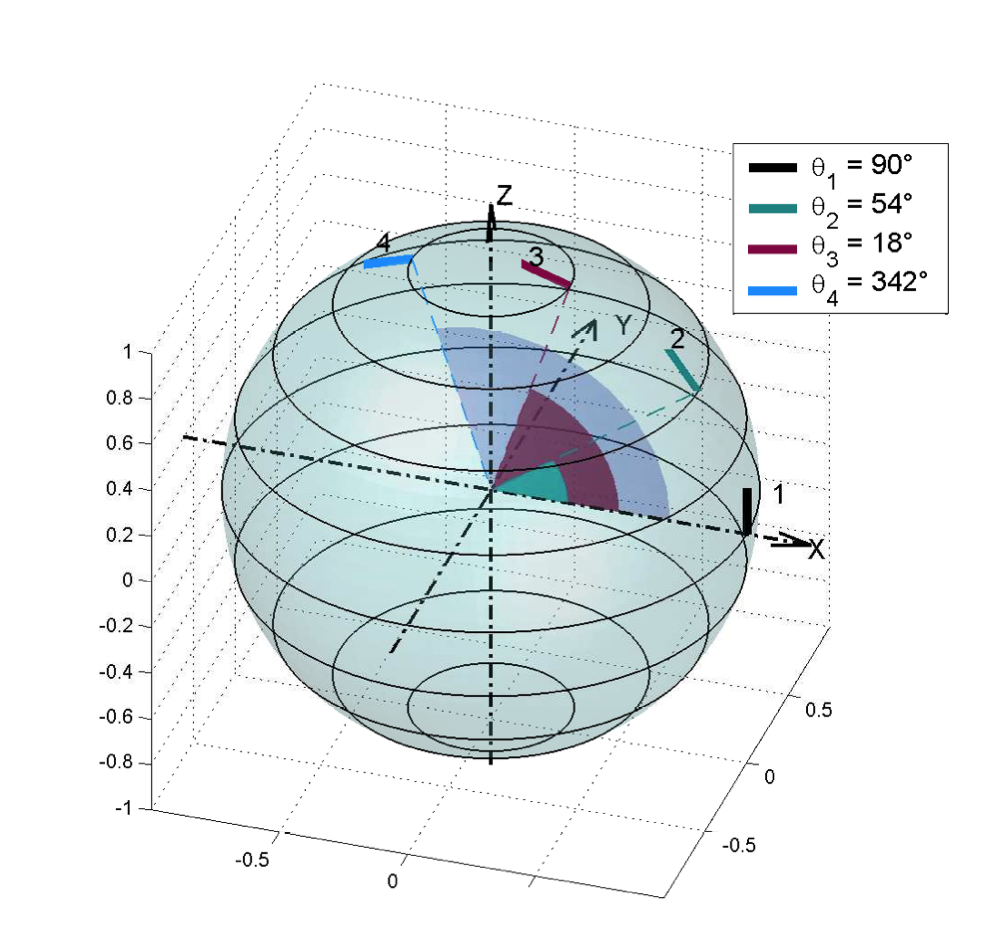
\includegraphics[width=0.49\textwidth]{img/eadf/measure.png}
    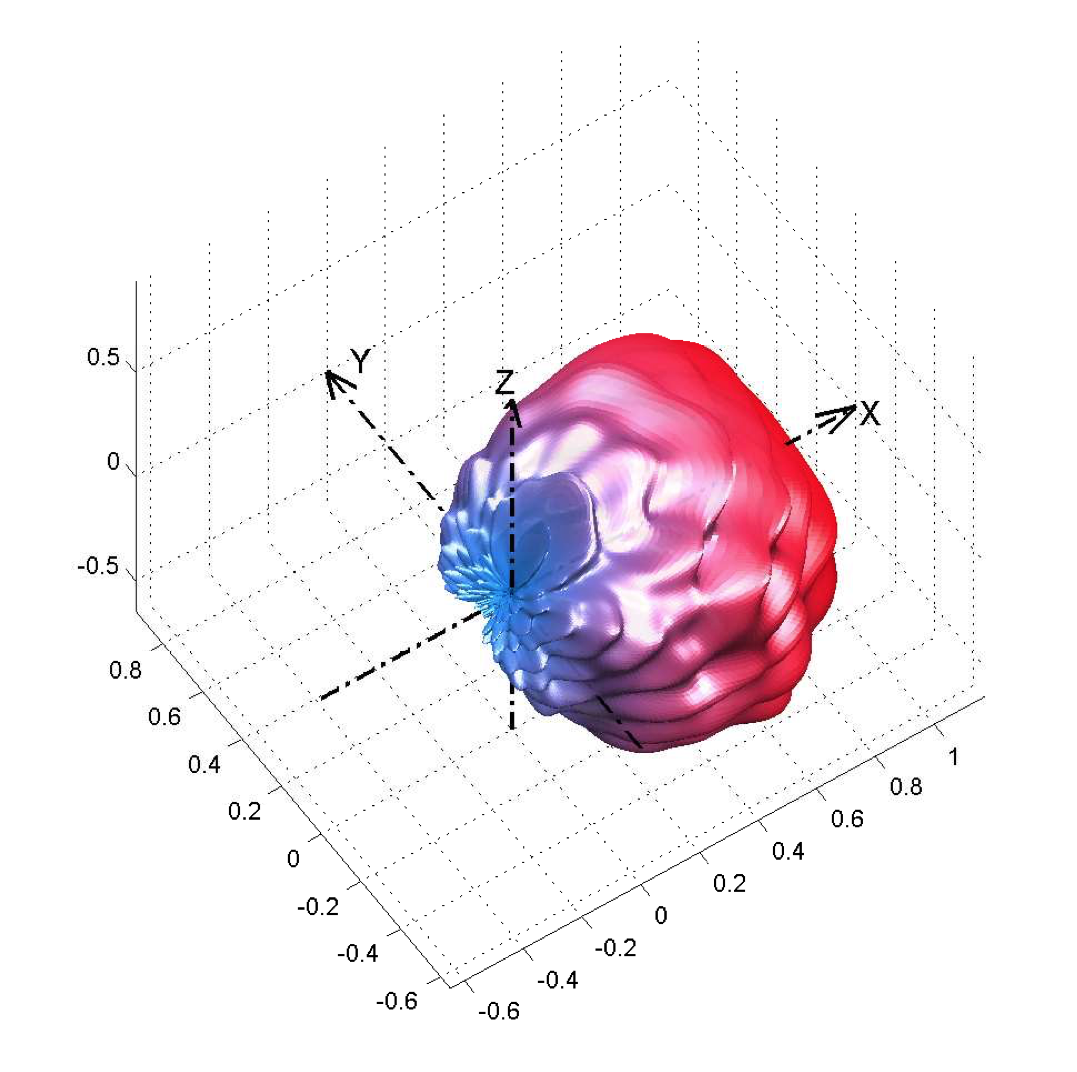
\includegraphics[width=0.49\textwidth]{img/eadf/3d_bp.png}
    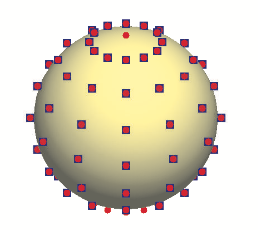
\includegraphics[width=0.3\textwidth]{img/eadf/bp_sampling.png}
    \caption{Links Oben: Darstellung der Messpositionen f\"ur eine Antenne, oder eine Antennenstruktur, welche sich im Ursprung des abgebildeten Koordinatensystems befindet. Rechts Oben: Darstellung der winkelabh\"angigen Amplitude eines einzelnen Patch-Elements. Unten: Messpunkte f\"ur die Abtastung der Funktion $a$. Grafiken aus \cite{landmann2004EADF,delgaldo2007phd}.}\label{eadf_meas}
\end{figure}

Das hei{\ss}t weiterhin, dass es uns m\"oglich ist, die Antenne an diskreten Stellen abzutasten, sodass wir mit der Annahme der Bandbegrenzung und der Aussage des Nyquist-Theorems ein Modell ableiten k\"onnen, welches die Antenne vollst\"andig charakterisiert. In diesem Sinne geht es darum die kontinuierliche Antennenantwort $a$ zu ``digitalisieren''. Die ``Abtastung'' erfolgt demnach im Winkelbereich. Der zugeh\"orige ``Frequenzbereich'' ist entsprechend der \emph{r\"aumliche Frequenzbereich}. \Cref{eadf_meas} zeigt einerseits schematisch den Messaufbau, das genutzte Koordinatensystem und beispielhaft die 3D-Darstellung einer Antennenantwort eines einzelnen Patch-Elements.

Die Messung selbst erfolgt in einer echofreien Messkammer, in welcher es m\"oglich ist, die \gls{aut} beliebig relativ zu einer bereits kalibrierten Referenzantenne zu verdrehen, sodass ein Abtastraster, wie in \Cref{eadf_meas} unten gezeigt, entsteht. Pro Ausrichtung wird die \gls{aut} f\"ur gew\"ohnlich f\"ur mehrere Frequenzen, zwei orthogonale Polarisationen und alle ihre Elemente vermessen, bevor die n\"achste Ausrichtung angefahren wird. Wie erw\"ahnt konzentrieren wir uns auf eine einzelne Frequenz, ein einzelnes Element und eine seiner Polarisationen.
In \Cref{eadf_anechoic} sieht man den Messaufbau, der von unserem FG benutzt wurde, um ein Antennenarray mit 32 Elementen zu vermessen.

\begin{figure}[t]
    \centering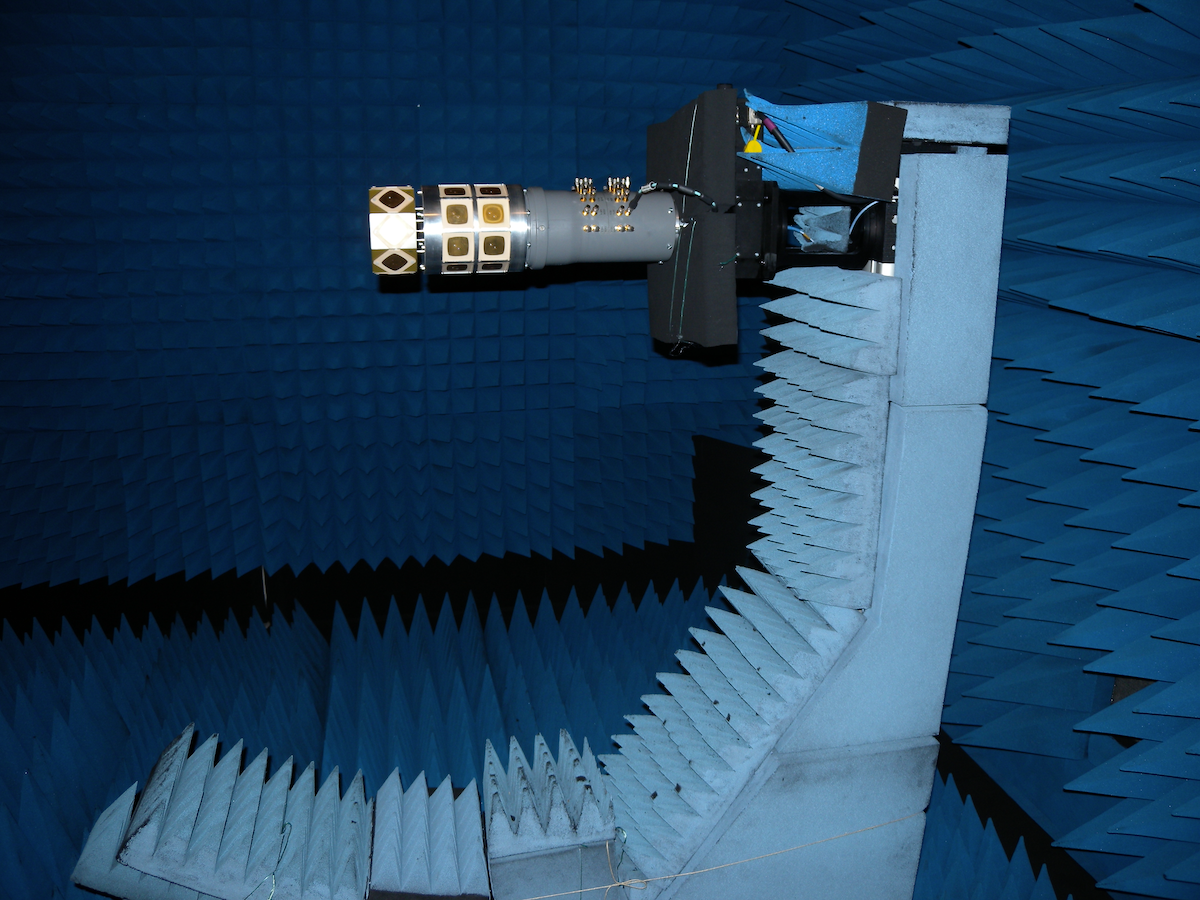
\includegraphics[width=0.49\textwidth]{img/eadf/anechoic1.png}
    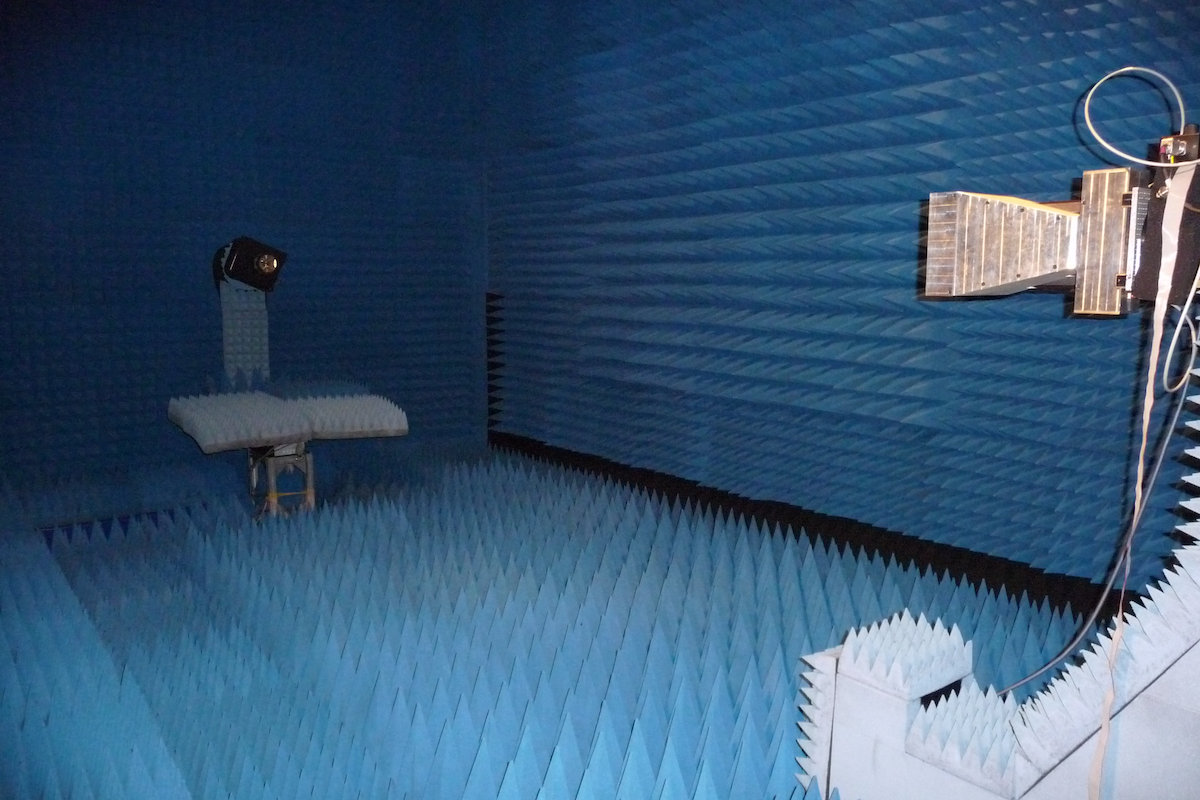
\includegraphics[width=0.49\textwidth]{img/eadf/anechoic2.png}
    \caption{Messaufbau zur Kalibrierung eines Antennenarrays. Links: Drehteller f\"ur die Positionierung der \gls{aut}. Rechts: Weiterer Blickwinkel mit Referenzantenne.}\label{eadf_anechoic}.
\end{figure}

F\"ur ein einzelnes Antennenelement beobachten wir also die Funktion $a$ auf einem Gitter, das aus allen Kombinationen der Punkte 
\[
    \varphi_0, \dots, \varphi_{N_\varphi}, \varphi_i = \frac{i \pi}{N_\varphi}
    \Text{und}
    \vartheta_0, \dots, \vartheta_{N_\vartheta-1}, \vartheta_j = \frac{j 2 \pi}{N_\vartheta}
\]
besteht. Wir erhalten also ein zweidimensionales Array $a[i,j] \in \C^{N_\varphi \times N_\vartheta - 1}$, welches wir noch durch einen Trick geeignet periodifizieren m\"ussen, wie in \cref{eadf_bp_aperture} links dargestellt. Diese Abtastwerte entspringen also einer zweidimensionalen bandbegrenzten, periodischen Funktion. Aufgabe ist es nun aus diesen Werten eine geeignete Interpolante herzuleiten, die sich diese beiden Eigenschaften zunutze macht.
%
%
\subsubsection{Fourier-Interpolation}
%
%
Gegeben sei ein periodisches, analoges Signal $x: \R \rightarrow \C$, mit periode $T_p = 1/F_0$. Wir beobachten dieses Signal auf einem uniformen Raster von Punkten, via $x[n] = x(n T)$ und wollen eine Funktion $y(t)$ herleiten, f\"ur welche die Interpolationsbedingung
\begin{equation}\label{eadf_interpol_cond}
    y(nT) = x[n] = x(nT)
\end{equation}
erf\"ullt ist. Hier zu entwickeln wir das Signal $x$ in seine Fourier-Reihe via
\begin{equation}\label{fourier_series}
    x(t) = \Sum{k=-\infty}{+\infty}{
        c[k] \exp(\jmath 2 \pi k t F_0) 
    }.
\end{equation}
Nun tasten wir dieses Signal uniform mit Samplerate $F_s = N/T_p = 1/T$ (also passend zur Periodendauer) ab und erhalten die Folge 
\begin{equation}
    x[n] = x(n T) = \Sum{k=-\infty}{+\infty}{
        c[k] \exp(\jmath 2 \pi k n T F_0) 
    } = \Sum{k=-\infty}{+\infty}{
        c[k] \exp\left(\jmath 2 \pi k \frac nN\right) 
    }
    \Text{f\"ur}
    n \in \N
\end{equation}
bestehend aus den Samples von $x$. Mit der Periodizit\"at von $\exp(\jmath 2 \pi t)$ und der Abtastung erhalten wir au{\ss}erdem noch
\begin{equation}
    x[n] = \Sum{k=0}{N-1}{
        \left[\Sum{\ell=-\infty}{+\infty}{
            c[k - \ell N]
        }\right] \exp\left(\jmath 2 \pi k \frac nN\right) 
    } = \Sum{k=0}{N-1}{
        \tilde{c}[k] \exp\left(\jmath 2 \pi k \frac nN\right) 
    },
\end{equation}
wobei wir 
\begin{equation}\label{aliased_ck}
    \tilde{c}[k] = \Sum{\ell=-\infty}{+\infty}{
        c[k - \ell N]
    }
\end{equation}
als Abk\"urzung benutzt haben. Ist nun die Funktion $x$ auch bandbegrenzt, d.h.~ihre Fourier-Transformierte $X : \R \rightarrow \C$ verschwindet au{\ss}erhalb eines gewissen Bandes, also
\begin{equation}
    X(F) = \Int{-\infty}{+\infty}{x(t) \exp(-\jmath 2 \pi F t )}{t} = 0 \Text{f\"ur} \Abs{F} > B.
\end{equation}
Au{\ss}erdem wissen wir, dass die Fourier-Transformation $X$ und die Folge $c[k]$ verkn\"upft sind via 
\begin{equation}
    c[k] = \frac{1}{T_p} X(k F_0),
\end{equation}
was impliziert, dass die Folge $c[k]$ verschwindet, also gilt
\begin{equation}
    c[k] = 0 \Text{f\"ur} \Abs{k} > \frac{B}{F_0}.
\end{equation}
Das hei{\ss}t, dass wir nun $F_s = N/T_p$ so gro{\ss} w\"ahlen m\"ussen, dass sich in \eqref{aliased_ck} kein Aliasing f\"ur $\tilde{c}[k]$ ergeben darf. Es muss also gelten
\begin{equation}
    N > \lceil B/F_0 \rceil \Text{bzw.} F_s > \lceil B/(F_0 T_p) \rceil.
\end{equation}
In diesem Falle gilt, dann dass $c[k] = X[k]$, wobei $X[k]$ die \gls{dft} der Folge $x[n]$ darstellt. Das hei{\ss}, dass wir die Fourier-Koeffizienten der kontinuierlichen Funktion $x$ durch die \gls{dft} der Abtastwerte $x[n]$ bestimmen k\"onnen. Mit \eqref{fourier_series} k\"onnen wir also die Folge $x[n]$ interpolieren, indem wir
\begin{equation}\label{dft_interpolation}
    y(t) = \frac{1}{T_p}\Sum{k=-\frac{B}{F_0}}{+\frac{B}{F_0}}{
        X[k] \exp(\jmath 2 \pi k t F_0) 
    }
\end{equation}
schreiben. Dieses $y$ erf\"ullt die Interpolationsbedingung \eqref{eadf_interpol_cond}, weil wegen der Bandbegrenzung von $x$ und der Periodizit\"at sogar gilt $y(t) = x(t)$ f\"ur alle $t$ gilt.

Man beachte hier, dass nun aus der Folge von diskreten Werten $x[n]$ eine analytische Formel in Form einer \emph{endlichen} Summation entstanden ist. Unter der Annahme der Bandlimitierung von $x$ ist diese Interpolation \emph{exakt} und kann effizient implementiert werden, durch die Vorberechnung der Folge $X[k]$ durch die \gls{fft}~\cite{FFTW05} der Folge $x[n]$. 
%
%
%
%
\subsubsection{Ableitung der EADF}
%
%
Wir wollen nun \eqref{dft_interpolation} auf zwei Dimensionen erweitern und folgen damit effektiv~\cite{landmann2004EADF}.
Au{\ss}erdem \"andern wir das Argument der Funktion $x$ und deren Namen zu der oben eingef\"uhrten Schreibweise $a : [0, 2 \pi] \times [0, 2 \pi] \rightarrow \C$ mit Werten $a(\varphi, \vartheta)$. 
In unserem Fall der Interpolation von Antennenantworten wissen wir, dass $a$ in \emph{beiden} Argumenten $2\pi$-periodisch ist.

\begin{figure}[t]
    \centering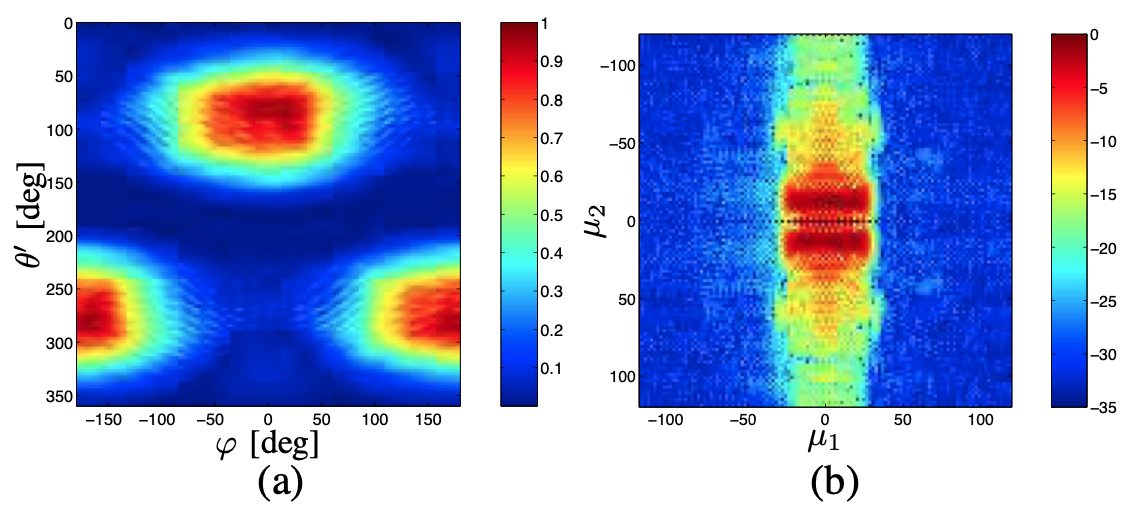
\includegraphics[width=0.75\textwidth]{img/eadf/bp_aperture.png}
    \caption{Links: Periodifizertes 2D Array $a[n_\varphi, n_\vartheta]$ der gemessenen Amplituden eines einzelnen Patch-Elements. Rechts: Der Betrag der zugeh\"origen \gls{eadf}, wobei hier $\mu_1 = k_\varphi$ und $\mu_2 = k_\vartheta$. Grafik aus~\cite{landmann2004EADF}}\label{eadf_bp_aperture}
\end{figure}

Die Bandlimitierung von $a$ l\"asst sich formulieren, indem man fordert, dass die Bedingungen
\begin{align}
    A_{\varphi}(F_\varphi, \vartheta) 
    &= \Int{-\infty}{+\infty}{
        a(\varphi, \vartheta) \exp(\jmath 2 \pi F_\varphi \varphi)
    }{\varphi} = 0 
    \fuer F_\varphi > B_\varphi \Text{und alle} \vartheta \in [0, 2 \pi] \Text{und} \\
    A_{\vartheta}(\varphi, F_\vartheta) 
    &= \Int{-\infty}{+\infty}{
        a(\varphi, \vartheta) \exp(\jmath 2 \pi F_\vartheta \vartheta)
    }{\varphi} = 0 
    \fuer F_\vartheta > B_\vartheta \Text{und alle} \varphi \in [0, 2 \pi]
\end{align}
erf\"ullt sein m\"ussen. Nun lassen sich alle obigen Argumente ``schnittweise'' auf eine abgetastete Version von $a$ in der Form $a[n_\varphi, n_\vartheta]$ anwenden. Das hei{\ss}t, wir landen schlussendlich bei einer Interpolations-Formel
\begin{equation}\label{2d_dft_interpolation}
    a(\varphi, \vartheta) = \Sum{k_\varphi=-\frac{B_\varphi}{F_\varphi}}{+\frac{B_\varphi}{F_\varphi}}{
        \Sum{k_\vartheta=-\frac{B_\vartheta}{F_\vartheta}}{+\frac{B_\vartheta}{F_\vartheta}}{
            A[k_\varphi, k_\vartheta] 
            \cdot \exp(\jmath 2 \pi k_\varphi \varphi F_\varphi)
            \cdot \exp(\jmath 2 \pi k_\vartheta \vartheta F_\vartheta)
        }
    },
\end{equation}
welche eine absolut analoge (nicht als Gegenteil zu digitale) $2D$-Version zu \eqref{dft_interpolation} darstellt. Auch in diesem Fall, k\"onnen wir das $2D$-Array $A[k_\varphi, k_\vartheta]$ durch eine $2D$-\gls{dft}, bzw. der \gls{fft}~\cite{FFTW05}, von den uniformen Samples $a[n_\varphi, n_\vartheta]$ der Funktion $a$ effizient vorberechnen.

Um einen m\"oglichst effizienten Algorithmus f\"ur die Auswertung der Interpolante zu erhalten, sollte man \eqref{2d_dft_interpolation} geeignet umschreiben. Moderne Rechenarchitekturen und Scientific-Computing-Libraries sind auf schnelle Matrix-Vektor-Produkte optimiert. Nehmen wir an, wir wollen \eqref{2d_dft_interpolation} f\"ur mehrere Winkelpaare $(\varphi_1, \vartheta_1), \dots, (\varphi_L, \vartheta_L)$ auswerten. Dann berechnen wir zun\"achst zwei $2D$ Arrays
\begin{align}
    D_\varphi &= [\exp(\jmath 2 \pi k_\varphi \varphi F_\varphi)]_{\ell = 1, k_\varphi=-\frac{B_\varphi}{F_\varphi}} \in \C^{L \times 2 \frac{B_\varphi}{F_\varphi} + 1} \Text{und}\\
    D_\vartheta &= [\exp(\jmath 2 \pi k_\vartheta \vartheta F_\vartheta)]_{\ell = 1, k_\vartheta=-\frac{B_\vartheta}{F_\vartheta}} \in \C^{L \times 2 \frac{B_\vartheta}{F_\vartheta} + 1}, 
\end{align}
was uns erlaubt \eqref{2d_dft_interpolation} in das folgende Vektor-Matrix-Vektor-Produkt
\begin{equation}\label{fast_2d_dft}
    a(\varphi_\ell, \vartheta_\ell) = 
        D_\varphi[\ell, :] \cdot A[:,:] \cdot D_\vartheta[\ell, :]^\trans
\end{equation}
umzuschreiben. Damit besteht der Interpolations-Algorithmus zun\"achst aus der Vorberechnung des Arrays $A$, sowie bei Ausf\"uhrung dann aus der Berechnung von $D_\varphi$ und $D_\vartheta$, sowie der Auswertung von \eqref{fast_2d_dft}.

Man sieht hier der sch\"on, dass die Laufzeitkomplexit\"at von \eqref{fast_2d_dft} ma{\ss}geblich von der r\"aumlichen Bandbegrenzung der Antennen-Richtcharakteristik beeinflusst wird. Je h\"oher die Bandbreite, desto h\"oher ist nicht nur der Aufwand bei der Messung, sondern auch bei der Interpolation. Eine alternative Form der Interpolation, welche diese eventuell nachteilige Eigenschaft nicht hat, ist in \Cref{b-splines} dargestellt.
